\documentclass{article}
\usepackage{graphicx}
\usepackage[english]{babel}
\usepackage{fancyvrb}
\usepackage{tikz}
\usetikzlibrary{shapes}

\title{Advanced topics}
\date{}

\begin{document}

\maketitle
\tableofcontents

\section{Overview}
This document goes into more advanced notions. It is intended for those wanting to understand what is happening behind the scenes, or who want to contribute to the project. It is \textbf{not} intended for end-users.

\section{Running The Sleeping Lion on Linux}
The general way of using The Sleeping Lion on Linux is by running the command \verb#thesleepinglion#. This will show the graphical interface.

However, one can also bypass the user interface by specifying a GML file to parse. Additionnaly, one can also give a target path to which the PDF file will be saved (if this path is not given, the resulting PDF will be placed at the same location as the GML file). For example, one can run:

\verb`thesleepinglion Spellweaver.gml` (will create the "Spellweaver.pdf" file)

\verb`thesleepinglion path/to/gml path/to/pdf`

\section{In depth study of the GML format}
\subsection{Overall structure and syntax}
A GML file can essentially be divided into three parts:
\begin{itemize}
	\item a part where you will be defining a few general properties about the custom class you are creating, such as the background color used for the cards or the class's symbol
	\item a part where you will be defining each card separatly. For each card, you will be filling out fields corresponding to the name of the card, the initiative, the actions in the top part of the card...
	\item shortcuts to make writing a GML file even easier (aliases).
\end{itemize}

Whenever writing a GML file, you will often be assigning values to certain fields: if you already know YAML, JSON, Ansible or RAML, then this should feel familiar: in fact, the GML format is built on YAML. The general way to do this is by using the following syntax: \verb`field: value`.
For example, when writing down the properties of a card, you will have to write \verb`initiative: 14` if you want the card to display an initiative of 14. Note that the fields must have a specific name: The Sleeping Lion will not recognise the words \verb`initiativ`, \verb`initiatve` or any other word which hasn't been thought of when designing the parser. Finally, note that \textbf{no field is mandatory} in GML. The cards may be a bit ugly, but there is no field that you must write down for the parser to work properly.

In GML, indentation matters.  The identation in itself should always be the same and should be of 2 blank spaces: its presence or absence matters. Writing the following
\begin{center}
\begin{BVerbatim}
initiative: 14
level: 1
\end{BVerbatim}
\end{center}

or

\begin{center}
\begin{BVerbatim}
initiative: 14
  level: 1
\end{BVerbatim}
\end{center}
does not mean the same thing, and can generate errors.

\textit{Note}: When using the graphical interface, The Sleeping Lion replaces every tab by two white spaces. When editing manually a GML file, take care to add only white spaces (two white spaces per level on indentation) and not tabs.

Overall, your GML file should have the following structure.
\begin{center}
\begin{BVerbatim}
class:
  field1: value1
  field2: value2
    ...

card_name1:
  field1: value1
  field2: value2
    ...

card_name2:
  field1: value1
  field2: value2
    ...
...

aliases:
  field1: value1
  field2: value2
    ...
\end{BVerbatim}
\end{center}

Note the indentation, and the colons. Detailed information about each part (class, cards and aliases) is given in the following sections.

\subsection{General class properties}
The first part allows you to define a few class-defining parameters such as the background color for cards. Here is how you would write those properties for the Spellweaver.
\begin{center}
\begin{BVerbatim}
class :
  name: Spellweaver
  color: 125,0,125
  path_to_icon: path/to/icon/
\end{BVerbatim}
\end{center}
Let's break down each line in this example:
\begin{itemize}
	\item \verb`class` means you are defining the global properties for this class. Note that every other value in this part is indented one level compared to the keyword \verb`class`.
	\item \verb`name` is the name of your class.
	\item \verb`color` is the background color used for every card for your class. You should write three values between 0 and 255, separated by comas. These values correspond to the RGB (red, blue, green) color used for your card.
	\item \verb`path_to_icon` is the path to an image (preferably a .svg file, but you can also put a .png) which will be used as an icon for your class and will be displayed at the bottom of every card. The path should be a relative path from the gml file (something like \verb`../../Gloomhaven/icon.svg`).
\end{itemize}

\subsection{Creating cards}
You may now create as many cards as you want. Each card should have the following syntax:
\begin{center}
\begin{BVerbatim}
Fire Orbs:
  level: 1
  initiative: 69
  ID: 061
  top: |2
    \attack{3}
    ...
  bottom: |2
    \move{3}
\end{BVerbatim}
\end{center}

Note that the names of the cards must be at the same indentation level as the keyword \verb`class`, defined in the section above.

Let's break down each line in this example:
\begin{itemize}
	\item \verb`Fire Orbs` is the name of the card we are currently creating. Note that every other value in this part is indented one level compared to the name of card.
	\item \verb`level` corresponds to the level of the card and will be shown at the top, in a small crown. You may also give letters, such that \verb`level: X` is valid.
	\item \verb`initiative` corresponds to the initiative of the card and will show in the middle. You may also give letters or numbers with more than two digits, although it may look ugly on the card.
	\item \verb`ID` corresponds to the card ID and will be shown in small at the bottom of the card. You may also give letters or numbers, such that \verb`S001` is valid.
	\item \verb`top` \textbf{must} be followed by the "pipe" symbol \verb`|` as well as the number \verb`2`. Also note that the text is again indented one level compared to the keyword \verb`top`. This is where you will be describing everything the top part of the card does. The syntax for describing the top (or bottom) half of a card is described in the tutorial.
	\item \verb`bottom` is the same as \verb`top` only the actions listed here will be displayed on the bottom of the card.
\end{itemize}

\subsection{Adding your own aliases}
The Sleeping Lion allows you to define your own aliases to write down simply your custom actions. To do this, simply add a new part to your GML file called aliases, as such:

\begin{center}
\begin{BVerbatim}
aliases: |
  custom_alias1 = something
  ...
\end{BVerbatim}
\end{center}

Note the "pipe" symbol \verb'|' after the keyword \verb'aliases'. You may define as many aliases as you wish: each alias should be on its own line.

\textit{Note}: to allow a better understanding of your cards to someone reading your GML file, it is highly recommended to put the \verb`aliases` section at the top of your GML file.

\pagebreak
\section{Pixel coordinates to hexagon coordinates}
This section describes some conventions used by the \verb`HexagonalGrid` class to draw a hexagonal grid and allow users to select a specific hex. Hexagons are regular, so the only parameter is $a$ the length of a side of a hexagon.

\subsection{Three sets of coordinates}
The \verb`HexagonalGrid` class draws hexagons using the pointy-top orientation. Furthermore, we use offset coordinates with an "even-r" layout meaning even rows are shoved right.

There are three sets of coordinates which we will be using:
\begin{itemize}
\item hexagonal coordinates, two integers encoding columns and rows following the above conventions. In this document, hexagonal coordinates are represented in italics, for example \textit{(0,0)}.
\item internal pixel coordinates, spanning from the orthonormal basis of the plane represented in red in the figure below. The origin (0,0) corresponds to the top left vertex of the hexagon with hexagonal coordinates \textit{(0,0)}. Note that the y-axis is pointing downwards, following cairo's conventions. In this document, internal pixel coordinates are represented using the default font, for example (0,0).
\item item coordinates, spanning from the same basis as internal pixel coordinates, but shifted. This basis is represented in blue in the figure below. The Sleeping Lion sees items as rectangular boxes: when drawing a box totally encompassing an AOE, the top left corner of the box does not correspond to the the origin of the internal pixel coordinates basis. Note that just like the previous basis, the y-axis is pointing downwards.
\end{itemize}

\begin{center}
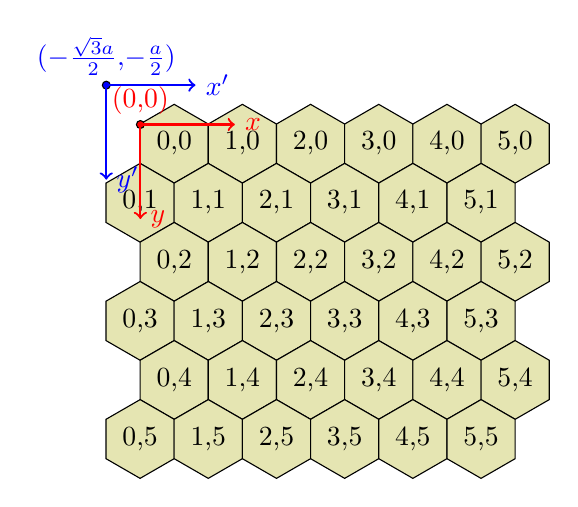
\begin{tikzpicture} [hexa/.style= {shape=regular polygon,regular polygon sides=6,minimum size=1cm, draw,inner sep=0,anchor=south,fill=lightgray!120!blue,rotate=30}]
\foreach \j in {0,...,5}{%
  \foreach \i in {0,...,5}{%
  \node[hexa] (h\i;\j) at ({\i*sin(60) - sin(60)/2 * Mod(\j,2) +0.75*sin(60)},{-\j*0.75 - 0.625}) {};}  }
  
\foreach \j in {0,...,5}{%
  \foreach \i in {0,...,5}{%
  \node [black] at (h\i;\j) {\i,\j};}  }
 f 
\draw[fill=red] (0,0) circle (0.05) node[above, text=red] {(0,0)};
\draw[->, thick, red] (0,0)--(1.2,0) node[right, text=red]{$x$};
\draw[->, thick, red] (0,0)--(0,-1.2) node[right, text=red]{$y$};

\draw[fill=blue] ({-sqrt(3)/4},0.5) circle (0.05) node[above, text=blue] {($-\frac{\sqrt{3}a}{2}$,$-\frac{a}{2}$)};
\draw[->, thick, blue] ({-sqrt(3)/4},0.5)--(0.7,0.5) node[right, text=blue]{$x'$};
\draw[->, thick, blue] ({-sqrt(3)/4},0.5)--({-sqrt(3)/4},-0.7) node[right, text=blue]{$y'$};
\end{tikzpicture}

The three sets of coordinates used
\end{center}

Note that converting coordinates between the two basis of the plane is quite simple, as it is simply a translation: hence we will be working in the internal pixel coordinates (in red in the figure above). The \verb`get_origin_pixel_coordinates` function computes this translation.

\subsection{Computing a clicked hexagon's hexagon coordinates}
Say the user clicks on a point $(x,y)$: how can we find the correspond clicked hexagon's coordinates?

We define $q_x$ and $r_x$ as $$x = q_x*\lfloor \sqrt{3}a\rfloor + r_x$$. Similarly, we define $q_y$ and $r_y$ as $$y = q_y*\lfloor \frac{3a}{2}\rfloor + r_y$$.

Defining $r_x$ and $r_y$ shifts the problem back into the hexagon \textit{(0,0)}, which makes reasoning easier.

\textbf{Remember that by cairo's convention, the y-axis is pointing downwards.}

\subsection{Computing clicked hexagon's column}
Given the position of a point $(x,y)$, how can we compute the clicked hexagon's column? First, let's split the hexagonal grid as shown in the figure below.

\begin{minipage}{0.45\linewidth}
\raggedleft
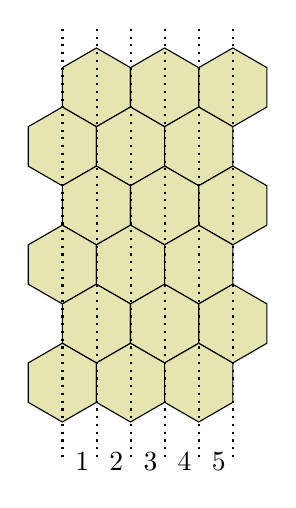
\begin{tikzpicture} [hexa/.style= {shape=regular polygon,regular polygon sides=6,minimum size=1cm, draw,inner sep=0,anchor=south,fill=lightgray!120!blue,rotate=30}]
\foreach \j in {0,...,5}{%
  \foreach \i in {0,...,2}{%
  \node[hexa] (h\i;\j) at ({\i*sin(60) - sin(60)/2 * Mod(\j,2) +0.75*sin(60)},{-\j*0.75 - 0.625}) {};}  }

\foreach \i in {0,...,5}{%
	\draw[-, dotted, thick] ({\i*sin(60)/2},{0.5})--({\i*sin(60)/2},{-5});}
\foreach \i in {1,...,5}{% Hack to be able to display 1...5 as labels and not 1...4
	\node [black] at ({0.25 + (\i-1)*sin(60)/2},{-5}) {\i};}
\end{tikzpicture}
\end{minipage}
\begin{minipage}{0.55\linewidth}
\raggedright
Notice that:
\begin{itemize}
\item if $x$ is in the column labeled "1", then it must be in column \textit{0}.
\item if $x$ is in the column labeled "2", it can be in column \textit{0} or \textit{1}.
\item if $x$ is in the column labeled "3", it must be in column \textit{1}.
\end{itemize}
\end{minipage}
We can also note that each column has the same width, which is $\frac{\sqrt{3}a}{2}$.

Therefore,
\begin{itemize}
\item if $r_x \leq \frac{\sqrt{3}a}{2}$, then point $(x,y)$ is in column $q_x$.
\item if $r_x \geq \frac{\sqrt{3}a}{2}$, then point $(x,y)$ is in column $q_x$ or $q_x +1$.
\end{itemize}

\subsubsection{Special case: $r_x \geq \frac{\sqrt{3}a}{2}$}
Once again, there are two possibilities according to the parity of $q_y$, illustrated in the figures below.

\begin{minipage}{0.45\linewidth}
\raggedleft
\begin{center}
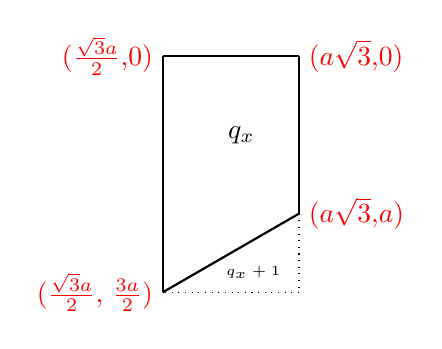
\begin{tikzpicture}
% hexagon_side = 2cm
\draw[-, thick] (0,0)--({sqrt(3)},0);
\draw[-, thick] ({sqrt(3)},0)--({sqrt(3)},-2);
\draw[-, thick] ({sqrt(3)},-2)--(0,-3);
\draw[-, thick] (0,-3)--(0,0);
\draw[-, dotted] ({sqrt(3)},-2)--({sqrt(3)},-3);
\draw[-, dotted] ({sqrt(3)},-3)--(0,-3);
\node [left, text=red] at (0,0) {($\frac{\sqrt{3}a}{2}$,0)};
\node [right, text=red] at ({sqrt(3)},0) {($a\sqrt{3}$,0)};
\node [right, text=red] at ({sqrt(3)},-2) {($a\sqrt{3}$,$a$)};
\node [left, text=red] at (0,-3) {($\frac{\sqrt{3}a}{2}$, $\frac{3a}{2}$)};
\node [black] at (1, -1) {$q_x$};
\node [black] at (1.15, -2.75) {\tiny $q_x+1$};
\end{tikzpicture}
\underline{Case 1:} $q_y$ is even.
\end{center}
\end{minipage}
\begin{minipage}{0.45\linewidth}
\raggedright
\begin{center}
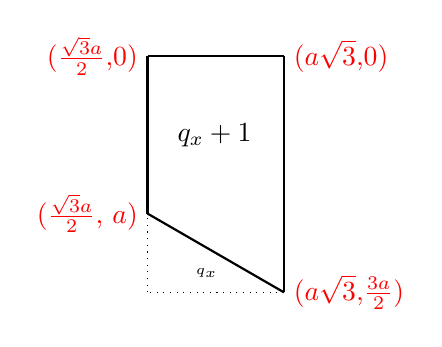
\begin{tikzpicture}
% hexagon_side = 2cm
\draw[-, thick] (0,0)--({sqrt(3)},0);
\draw[-, thick] ({sqrt(3)},0)--({sqrt(3)},-3);
\draw[-, thick] ({sqrt(3)},-3)--(0,-2);
\draw[-, thick] (0,-2)--(0,0);
\draw[-, dotted] ({sqrt(3)},-3)--(0,-3);
\draw[-, dotted] (0,-3)--(0,-2);
\node [left, text=red] at (0,0) {($\frac{\sqrt{3}a}{2}$,0)};
\node [right, text=red] at ({sqrt(3)},0) {($a\sqrt{3}$,0)};
\node [right, text=red] at ({sqrt(3)},-3) {($a\sqrt{3}$,$\frac{3a}{2}$)};
\node [left, text=red] at (0,-2) {($\frac{\sqrt{3}a}{2}$, $a$)};
\node [black] at (0.85, -1) {$q_x +1$};
\node [black] at (0.75, -2.75) {\tiny $q_x$};
\end{tikzpicture}
\underline{Case 2:} $q_y$ is odd.
\end{center}
\end{minipage}

\underline{Case 1: $q_y$ is even}

Note that if $r_y < a$, then the resulting column is $q_x$, since the point is located in the rectangle with coordinates $(\frac{\sqrt{3}a}{2}, 0)$ - $(a\sqrt{3}, 0)$ - $(a\sqrt{3}, a)$ - $(\frac{\sqrt{3}a}{2}, a)$.

We now assume that $r_y > a$.

First, we translate all points by $(a\sqrt{3},a)$. In this shifted basis, the problem can be summarized as:

\begin{center}
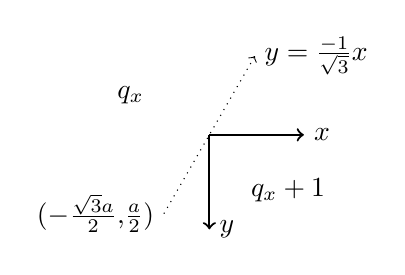
\begin{tikzpicture}
\draw[->, thick, black] (0,0)--(1.2,0) node[right]{$x$};
\draw[->, thick, black] (0,0)--(0,-1.2) node[right]{$y$};
\draw[->, dotted] ({-sqrt(3)/3},-1)--({sqrt(3)/3}, 1);
\node [below, left] at ({-sqrt(3)/3},-1) {($-\frac{\sqrt{3}a}{2}$,$\frac{a}{2}$)};
\node [black] at (1, -0.7) {$q_x +1$};
\node [black] at (-1, 0.5) {$q_x$};
\node [black, right] at ({sqrt(3)/3}, 1) {$y = \frac{-1}{\sqrt{3}}x$};
\end{tikzpicture}
\end{center}

Therefore, in the shifted basis, if $y \geq \frac{-1}{\sqrt{3}}x$, the column is $q_x+1$. Remember that cairo's convention is to have the y-axis pointing downwards.

\underline{Case 2: $q_y$ is odd}

Note that if $r_y < a$, then the resulting column is $q_x +1$, since the point is located in the rectangle with coordinates $(\frac{\sqrt{3}a}{2}, 0)$ - $(a\sqrt{3}, 0)$ - $(a\sqrt{3}, a)$ - $(\frac{\sqrt{3}a}{2}, a)$.

We now assume that $r_y > a$.

Here, we translate all points by $(\frac{\sqrt{3}a}{2},a)$. In this shifted basis, the problem can be summarized as:
\begin{center}
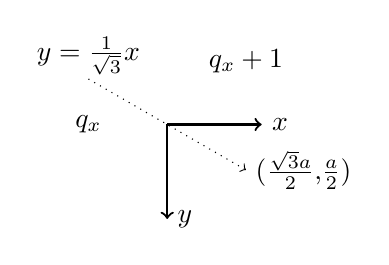
\begin{tikzpicture}
\draw[->, thick, black] (0,0)--(1.2,0) node[right]{$x$};
\draw[->, thick, black] (0,0)--(0,-1.2) node[right]{$y$};
\draw[->, dotted] (-1,{sqrt(3)/3})--(1,-{sqrt(3)/3});
\node [black] at (1, 0.8) {$q_x +1$};
\node [black] at (-1, 0) {$q_x$};
\node [above] at (-1, 0.5) {$y = \frac{1}{\sqrt{3}}x$};
\node [right] at (1,-{sqrt(3)/3}) {($\frac{\sqrt{3}a}{2}$,$\frac{a}{2}$)};
\end{tikzpicture}
\end{center}

Therefore, if $y \leq \frac{1}{\sqrt{3}}x$, the column is $q_x+1$.

\subsection{Computing clicked hexagon's line}
Like before, let's split the hexagonal grid as follow:


\begin{minipage}{0.45\linewidth}
\raggedleft
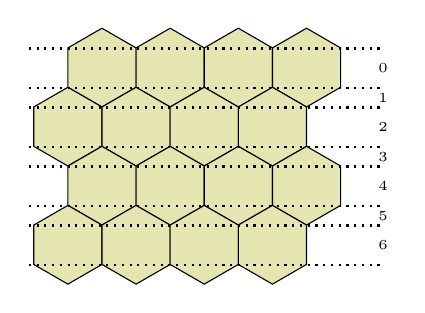
\begin{tikzpicture} [hexa/.style= {shape=regular polygon,regular polygon sides=6,minimum size=1cm, draw,inner sep=0,anchor=south,fill=lightgray!120!blue,rotate=30}]
\foreach \j in {0,...,3}{%
  \foreach \i in {0,...,3}{%
  \node[hexa] (h\i;\j) at ({\i*sin(60) - sin(60)/2 * Mod(\j,2) +0.75*sin(60)},{-\j*0.75 - 0.625}) {};}  }
	
\draw[-, dotted, thick] (-0.5, -0)--(4, -0);
\node [black] at (4, -0.25) {\tiny 0};
\draw[-, dotted, thick] (-0.5, -0.5)--(4, -0.5);
\node [black] at (4, -0.625) {\tiny 1};
\draw[-, dotted, thick] (-0.5, -0.75)--(4, -0.75);
\node [black] at (4, -1) {\tiny 2};
\draw[-, dotted, thick] (-0.5, -1.25)--(4, -1.25);
\node [black] at (4, -1.375) {\tiny 3};
\draw[-, dotted, thick] (-0.5, -1.5)--(4, -1.5);
\node [black] at (4, -1.75) {\tiny 4};
\draw[-, dotted, thick] (-0.5, -2)--(4, -2);
\node [black] at (4, -2.125) {\tiny 5};
\draw[-, dotted, thick] (-0.5, -2.25)--(4, -2.25);
\node [black] at (4, -2.5) {\tiny 6};
\draw[-, dotted, thick] (-0.5, -2.75)--(4, -2.75);
\end{tikzpicture}
\end{minipage}
\begin{minipage}{0.55\linewidth}
\raggedright

Notice that:
\begin{itemize}
\item if $y$ is in the line labeled "0", then it must be in line \textit{0}.
\item if $y$ is in the line labeled "1", it can be in line \textit{0} or \textit{1}.
\item if $y$ is in the line labeled "2", it must be in line \textit{1}.
\end{itemize}
\end{minipage}

Line have alternating width $a$ and $\frac{a}{2}$.
Therefore,
\begin{itemize}
\item if $r_y \leq a$, then point $(x,y)$ is in line $q_y$.
\item if $r_y \geq a$, then point $(x,y)$ is in line $q_y$ or $q_y +1$.
\end{itemize}

\subsubsection{Special case: $r_y \geq a$}
Like before, there are two possibilities, according to the parity of $q_y$:

\begin{minipage}{0.45\linewidth}
\raggedleft
\begin{center}
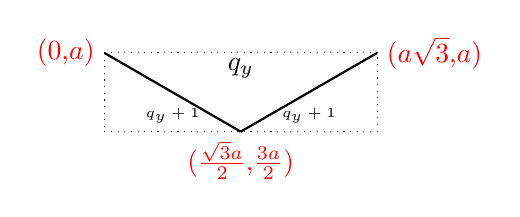
\begin{tikzpicture}
% hexagon_side = 2cm
\draw[-, dotted] (0,0)--({2*sqrt(3)},0);
\draw[-, thick] ({2*sqrt(3)},0)--({sqrt(3)},-1);
\draw[-, thick] ({sqrt(3)},-1)-- (0,0);
\draw[-, dotted] (0,0)--(0,-1);
\draw[-, dotted] (0,-1)--({2*sqrt(3)},-1);
\draw[-, dotted] ({2*sqrt(3)},-1) -- ({2*sqrt(3)},0);

\node [left, text=red] at (0,0) {(0,$a$)};
\node [right, text=red] at ({2*sqrt(3)},0) {($a\sqrt{3}$,$a$)};
\node [below, text=red] at ({sqrt(3)},-1) {($\frac{\sqrt{3}a}{2}$,$\frac{3a}{2}$)};
\node [black] at ({sqrt(3)}, -0.2) {$q_y$};
\node [black] at ({sqrt(3)/2}, -0.8) {\tiny $q_y+1$};
\node [black] at ({3*sqrt(3)/2}, -0.8) {\tiny $q_y+1$};
\end{tikzpicture}
\underline{Case 1:} $q_y$ is even.
\end{center}
\end{minipage}
\begin{minipage}{0.45\linewidth}
\raggedright
\begin{center}
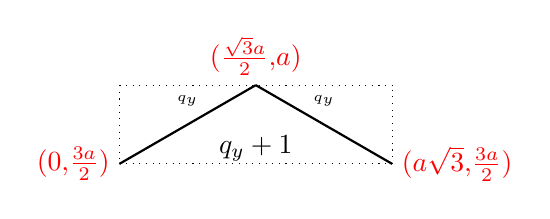
\begin{tikzpicture}
% hexagon_side = 2cm
\draw[-, dotted] (0,0)--({2*sqrt(3)},0);
\draw[-, thick] ({2*sqrt(3)},-1)--({sqrt(3)},0);
\draw[-, thick] ({sqrt(3)},0)-- (0,-1);
\draw[-, dotted] (0,0)--(0,-1);
\draw[-, dotted] (0,-1)--({2*sqrt(3)},-1);
\draw[-, dotted] ({2*sqrt(3)},-1) -- ({2*sqrt(3)},0);

\node [left, text=red] at (0,-1) {(0,$\frac{3a}{2}$)};
\node [right, text=red] at ({2*sqrt(3)},-1) {($a\sqrt{3}$,$\frac{3a}{2}$)};
\node [above, text=red] at ({sqrt(3)},0) {($\frac{\sqrt{3}a}{2}$,$a$)};
\node [black] at ({sqrt(3)}, -0.8) {$q_y+1$};
\node [black] at ({sqrt(3)/2}, -0.2) {\tiny $q_y$};
\node [black] at ({3*sqrt(3)/2}, -0.2) {\tiny $q_y$};
\end{tikzpicture}
\underline{Case 2:} $q_y$ is odd.
\end{center}
\end{minipage}

\underline{Case 1: $q_y$ is even}

It is easier to split the problem again and to reason according to $r_x$. More precisely, we can split the above shape into two vertically, such that we treat the cases $r_x \leq \frac{\sqrt{3}a}{2}$, and $r_x > \frac{\sqrt{3}a}{2}$ separately.

Like before, we then perform a translation so that we simply need to check on which side of a line the point $(x,y)$ lies.
\begin{itemize}
\item $r_x \leq \frac{\sqrt{3}a}{2}$: we translate by $(0,a)$. The result is $q_y+1$ if in this shifted basis, $y \geq \frac{1}{\sqrt{3}}x$
\item $r_x > \frac{\sqrt{3}a}{2}$: we translate by $(a\sqrt{3},a)$. The result is $q_y+1$ if in this shifted basis, $y \geq -\frac{1}{\sqrt{3}}x$
\end{itemize}

\underline{Case 2: $q_y$ is odd}

As previously, we split the problem in two vertically, then perform a translation.
\begin{itemize}
\item $r_x \leq \frac{\sqrt{3}a}{2}$: we translate by $(\frac{\sqrt{3}a}{2},a)$. The result is $q_y+1$ if in this shifted basis, $y \geq -\frac{1}{\sqrt{3}}x$
\item $r_x > \frac{\sqrt{3}a}{2}$: we translate by $(\frac{\sqrt{3}a}{2},a)$. The result is $q_y+1$ if in this shifted basis, $y \geq \frac{1}{\sqrt{3}}x$
\end{itemize}


\end{document}
